
\documentclass[11pt]{article}

%Menge: \mathbb{R}

\usepackage[ngerman]{babel}
\usepackage{amsmath} %align, für = untereinander einfach &=
\usepackage{amssymb}
\usepackage{amsthm}
\usepackage{listings}
\usepackage{pdfpages}
\usepackage[utf8]{inputenc}
\usepackage{graphicx}
\usepackage{esvect}
\graphicspath{ {./images/} }
\usepackage{tikz}         % For arrow and dots in \xvec
\usepackage[left=2.30cm, right=2.30cm, top=1.70cm, bottom=2.00cm]{geometry}

% --- Macro \xvec
\makeatletter
\newlength\xvec@height%
\newlength\xvec@depth%
\newlength\xvec@width%
\newcommand{\xvec}[2][]{%
	\ifmmode%
	\settoheight{\xvec@height}{$#2$}%
	\settodepth{\xvec@depth}{$#2$}%
	\settowidth{\xvec@width}{$#2$}%
	\else%
	\settoheight{\xvec@height}{#2}%
	\settodepth{\xvec@depth}{#2}%
	\settowidth{\xvec@width}{#2}%
	\fi%
	\def\xvec@arg{#1}%
	\def\xvec@dd{:}%
	\def\xvec@d{.}%
	\raisebox{.2ex}{\raisebox{\xvec@height}{\rlap{%
				\kern.05em%  (Because left edge of drawing is at .05em)
				\begin{tikzpicture}[scale=1]
				\pgfsetroundcap
				\draw (.05em,0)--(\xvec@width-.05em,0);
				\draw (\xvec@width-.05em,0)--(\xvec@width-.15em, .075em);
				\draw (\xvec@width-.05em,0)--(\xvec@width-.15em,-.075em);
				\ifx\xvec@arg\xvec@d%
				\fill(\xvec@width*.45,.5ex) circle (.5pt);%
				\else\ifx\xvec@arg\xvec@dd%
				\fill(\xvec@width*.30,.5ex) circle (.5pt);%
				\fill(\xvec@width*.65,.5ex) circle (.5pt);%
				\fi\fi%
				\end{tikzpicture}%
	}}}%
	#2%
}
\makeatother

% --- Override \vec with an invocation of \xvec.
\let\stdvec\vec
\renewcommand{\vec}[1]{\xvec[]{#1}}
% --- Define \dvec and \ddvec for dotted and double-dotted vectors.
\newcommand{\dvec}[1]{\xvec[.]{#1}}
\newcommand{\ddvec}[1]{\xvec[:]{#1}}

%eigene Befehle:
\newcommand{\R}{$\mathbb{R}$}

\title{Physik 1 Skript}
\date{\today}
\begin{document}
\lstset{language=Java}
\author{Tom Herrmann}

\maketitle

%Inhaltsverzeichnis
\tableofcontents

\newpage

\section{Einführung}
	peter.schleper@physik.uni-hamburg.de
	\subsection{Übungsgruppen}
		Es gibt 4 Übungsgruppe und eine davon ist auf Englisch.
	\subsection{Klausurbonus}
		Es müssen 50\%  der Aufgaben richtig abgegeben worden sein des jeweiligen Teils (Experimantal und theoretische Physik) um einen Klausurbonus zu erhalten.
		Der Klausurbonus ermöglicht es mit nur 30\% der benötigten Punktzahl die Klausur zu bestehen.
	\subsection{Buchempfehlungen}
		\textbf{Gerthsen} "Physik" Verlag Springer ist das Buch mit dem er gelernt hat.
\part{Vorlesung 1}
	\section{Was ist Experimentalpyhsik?}
	Die ersten Leute die sich gedanken in Richtung Physik gemacht haben waren Philosophen und erst ab dem 17 Jahrhundert fing der Umschwung an. 
	Dabei war der Gedanke einfach Erkenntnisse über die Natur zu erlangen und dies wenn möglich zu vereinfachen. Wie Einstein aber sagte: "Dinge zu vereinfachen ist gut, sie einfacher zu machen als sie eigentlich sind aber nicht"
 	\section{Was macht ein gutes Experiment aus?}
 		\begin{itemize}
 			\item Naturbeobachtung
 			\item reproduzierbar
 			\item Naturgesetzte daraus ableiten
 		\end{itemize}
	\section{SI-Einheiten}
		x = $1.307 m$ $\rightarrow$ Einheit $[x] \Rightarrow$ = Meter ; dim x = Länge definieren Standards
		\begin{itemize}
			\item $[$Zeit$]$ = SI: s - cgs: s
			\item $[$L\ddot{a}ngen$]$ = SI: m - cgs: cm
			\item $[$Masse$]$ = SI: kg - cgs: g
		\end{itemize}
		\subsection{Dimension}
	$[$Länge$] = 1m$\\
	$[$Fl\ddot{a}che$] = 1m^2$\\
	$[$Volumen$] = 1m^3$\\
	$[$Geschwindigkeit$] = 1\frac{m}{s}$\\
	$[$Zeit$] = 1s$\\
	$[$Kraft$] = 1N = 1\frac{kg\times m}{s^2}$\\
	$[$Leistung$] = 1W = 1\frac{N}{s^2} = 1\frac{kg\times m}{s^3}$\\
	Sämtliche Terme einer Gleichung müssen dem entsprechend die gleiche Dimension haben
\part{Vorlesung 2}
	\section{Wiederholung}
	Wichtige Faktoren für ein gutes Experiment
		\begin{itemize}
			\item Reduzierung von Naturerscheinungen
			\item Vereinfachung
			\item Systematisch
			\item Qualitativ
			\item Reproduzierbar
		\end{itemize}
\subsection{Definitionen}
 	Eine Sekunde wird am besten über die Atomphysik definiert und zwar über die Cs Atome.\\
 	Ein Meter ist über die Lichtgeschwindigkeit Definition. 1m = c * $\frac{1s}{299792458 m}$\\
 	Die Masse wird definiert über ein sogenanntes Urkilogramm. Sprich über eine Masse werden alle anderen Massen definiert.\\
 	Stromstärke: A wird ebenfalls über ein Experiment definiert.\\
 	Stoffmenge: mol\\
 	Temperatur: Kelvin \quad k\\
 	\textbf{Alle Naturkonstanten wurden letztes Jahr (2018) dabei neu definiert um eine höhere Genauigkeit zu gewährleisten}
\section{Kinematik des Massenpunktes}
 	Ein realer Körper:
 	\begin{itemize}
 		\item Translation
 		\item Rotation
 		\item Deformation
 	\end{itemize}
 Aber nun reden wir über einen starren Körper also einen Körper bei dem alle Abstände innerhalb des Körpers unabhängig von der Zeit gleich bleiben \textbf{(keine Deformation)}.\\
 Auf den Massepunkt wirkt ebenfalls keine Rotation in diesem Beispiel. Was allerdings nicht heißt dass man in der realen Welt die Rotation (SPIN) einfach vernachlässigen kann egal wie klein dieses Teilchen auch sein möge.\\
  \subsection{Behauptung}
  Man kann 2-Dimensionale Bewegungen beschreiben.
  	\begin{center}
  		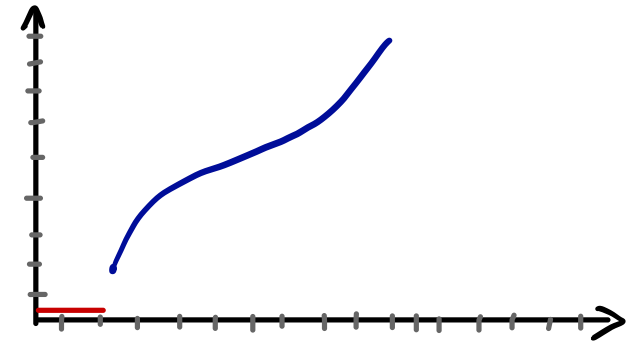
\includegraphics[scale=0.3]{20190411_073844099_iOS.png}
  		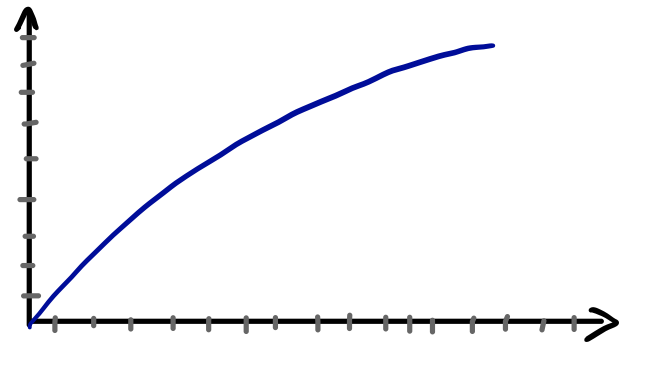
\includegraphics[scale=0.3]{20190411_074045495_iOS.png}
  		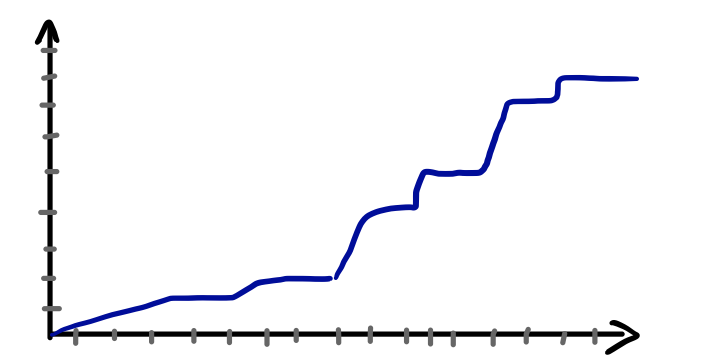
\includegraphics[scale=0.3]{20190411_074437642_iOS.png}
  		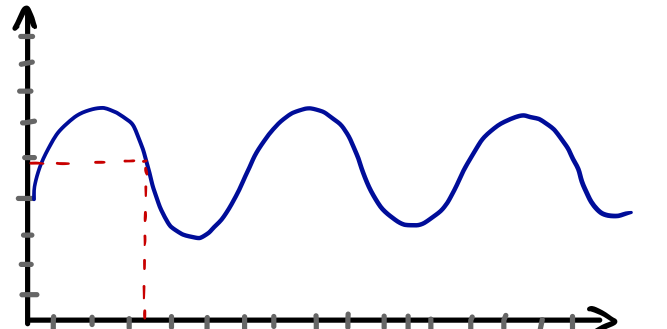
\includegraphics[scale=0.3]{20190411_074619898_iOS.png}\\
  	\textit{x-Achse = Zeit t; y-Achse= Position x}
  	\end{center}
 \subsection{1-dimensionale Bewegung}
 	\begin{center}
 			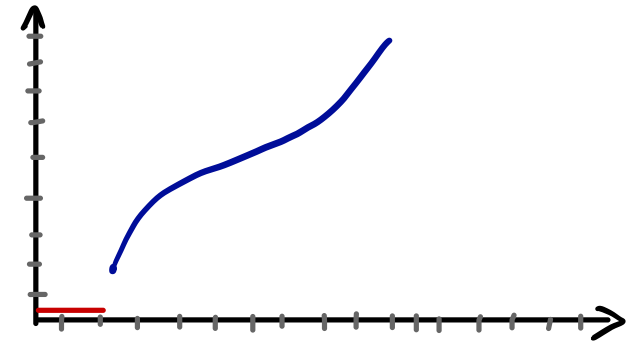
\includegraphics[scale=0.3]{20190411_073844099_iOS.png}
 	\end{center}
 \[ v = \frac{x_2 - x_1}{t_2 - t_1} = \frac{\Delta x}{\Delta t} \Leftrightarrow \lim_{\Delta t\to\ 0} \]
 Die Geschwindigkeit ist natürlich immer eine Durchschnittsangabe da es über eine gewisse Zeitspanne angeben wird. 
 
 \newpage
 \part{Vorlesung 3}
 			v = $\dot{x}$ \qquad v = $\frac{dx}{dt}$ \\
 			a = $\dot{v}$ = $\ddot{x}$ \qquad  a = $\frac{dv}{dt} = \frac{d^2x}{dt^2}$ \\
 			Mittelwerbeschleunigung = $\frac{\Delta x}{\Delta t} = \frac{\frac{x_4 - x_3}{t_4 - t_3} - \frac{x_2 - x_1}{t_2 - t_1}}{t_3 - t_1}$
  	\begin{center}
 	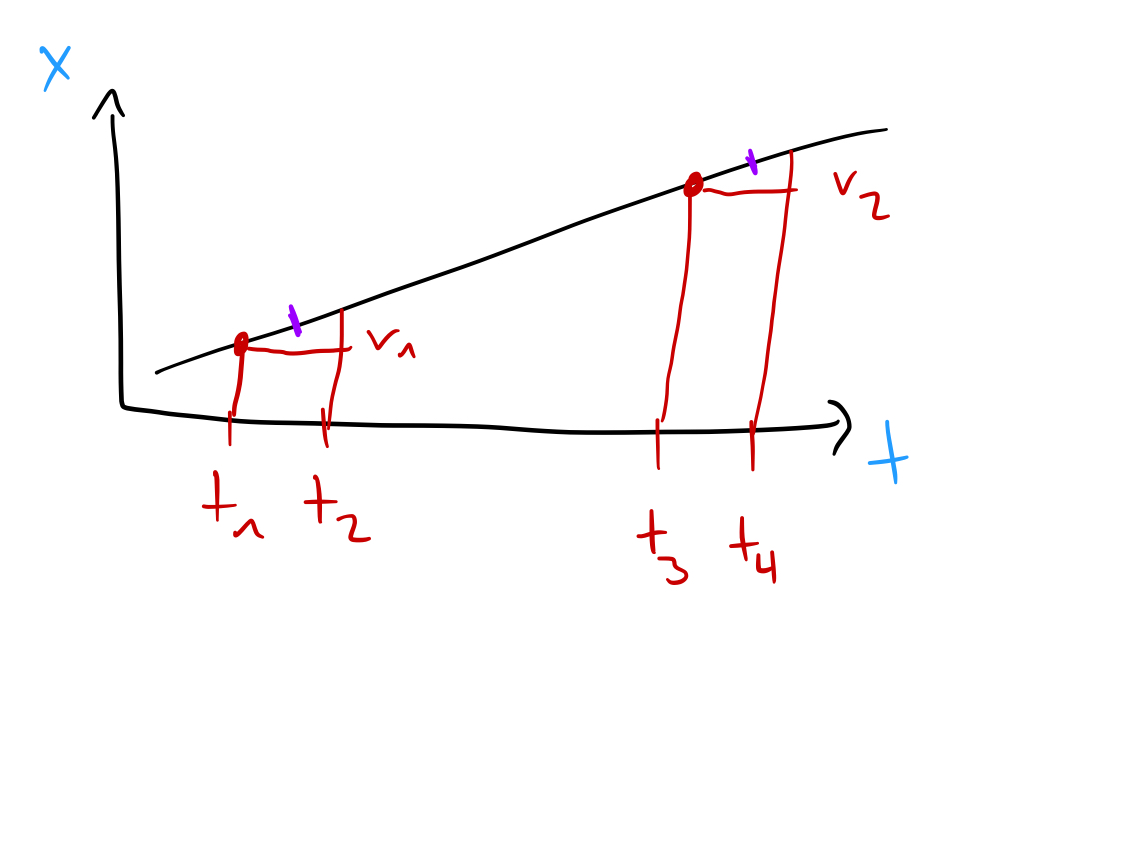
\includegraphics[scale=0.3]{IMG_EFF187166B54-1.jpeg}
 	\end{center}
 \[ v = \frac{dx}{dt} \rightarrow x_(t) = x_0 + \int_{t}^{t_0} v dt \]
\[ a = \frac{dv}{dt} \rightarrow v_(t)  = v_0 + \int_{t}^{t_0} a dt \]
	$x_(t)$ bei gegebenen $a(t)$ \\
		$x(t) = x_0 + \int_{t}^{t_0} (v_0 + \int_{t´´}^{t_0} a_(_t_) dt) dt´´$ \\
		
		$v(t)$ aus $a(x)$: \\
		v = $\frac{dx}{dt}$ \qquad dt = $\frac{dx}{v}$ \\
		a = $\frac{dv}{dt} $ \qquad dt = $\frac{dv}{a}$\\
		darauf ergibt sich $\frac{dx}{v} = \frac{dv}{a}$ $\Leftrightarrow \int_{v_1}^{v_0} v dv = \int_{x_1)}^{x_2} a_(x)dx$ durch weiteres umformen kommt man zum ausdruck: \\
		\[ \frac{1}{2} v^2 -\frac{1}{2} v_0^2 = \int_{x}^{x_0} a_(_x_)dx \]
 Wenn man nun die Masse mit einbezieht kommt man zur klassischen kinetischen Energie\\
  \[ \frac{1}{2} mv^2 - \frac{1}{2} mv^2 = \int_{x}^{x_0} a_(x) dx \]
  
  \section{3.3.4 Spezialfälle}
  	\subsection{Gleichförmige Bewegung}
  		a = 0  $\Leftrightarrow v = v_0$ \qquad $x_(_t_) = x_0 + v_0(t - t_0)$ \\
  		Also ist die Geschwindigkeit konstant 
	\subsection{konstante Beschleunigung}
			a = const \qquad $v = v_0 + a(t - t_0)$ \\
			$ x = x_0 + \int_{t_0}^{t} (v_0 + a(t - t_0))dt) \\
				= x_0 + \int_{t_0}^{t} v_0 dt + a \int_{t_0}^{t} (t - t_0) dt\\
				x = x_0 + v_0(t- t_0) + \frac{1}{2}a(t - t_0)^2 $ \\
			\textbf{Wahl des Koordinaten Systems:\\ t=0 und x=0}
			Gleichförmige Bewegung: $a = 0 ; v = v_0 \rightarrow x = v * t$ \\
			\textbf{konstante Beschleungung:} $a = const ; v = v_0 + a t ; x = vt + \frac{1}{2} at^2 $
\section{3.4 3-Dimensionale Bewegung (Vektoren)}
	  	\begin{center}
		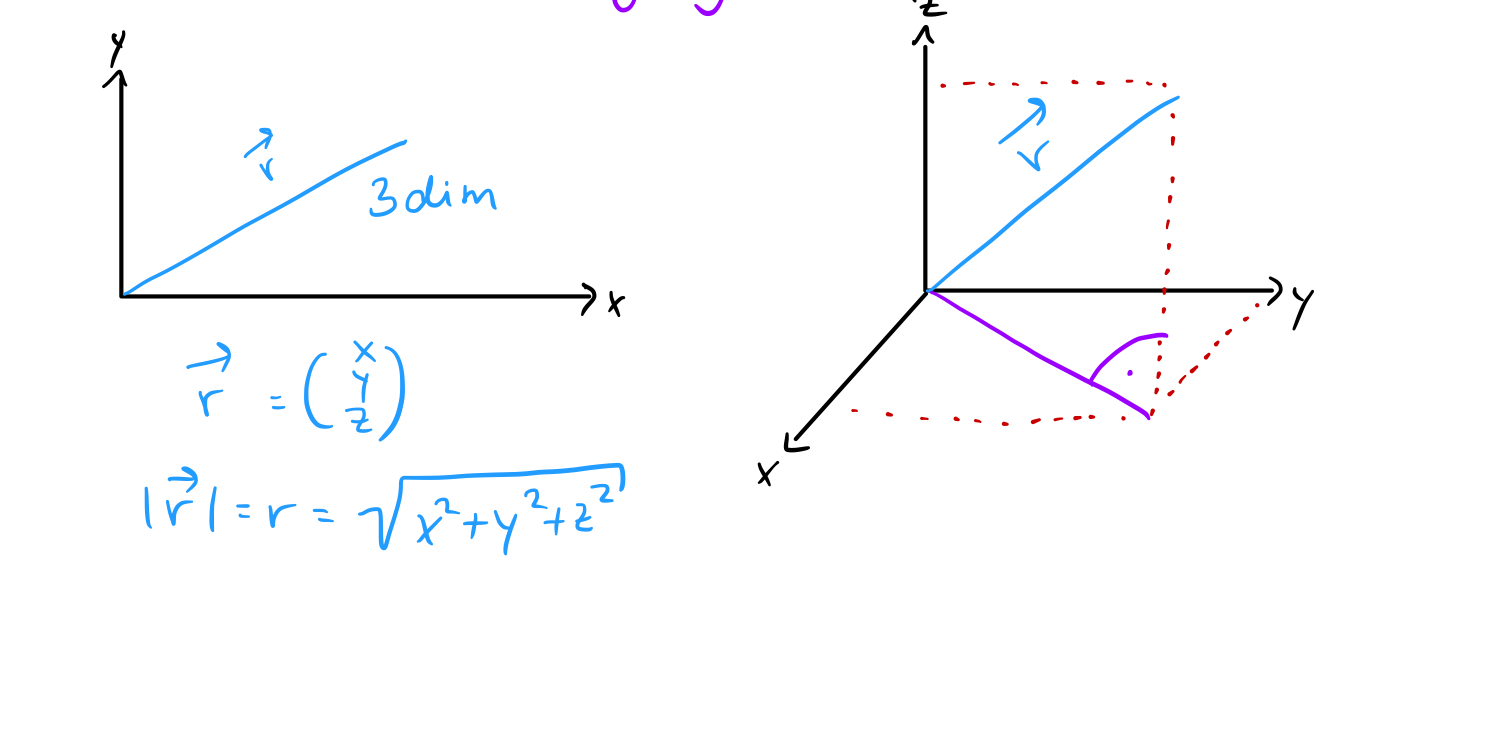
\includegraphics[scale=0.3]{IMG_8E3512F499A3-1.jpeg}
	\end{center}
	Sofern es keinen Vektorpfeil über einem Vektor gibt ist meist die Länge des Vektors gemeint\\
		$\vec{r} = \left(\begin{array}{cc}
		x \\
		y \\
		z
		\end{array} \right) $
		$\|\vec{r}\| = r = \sqrt{x^2 + y^2 + z^2}$ \\
		$\Leftrightarrow v_x = \frac{dx}{dt}$ \qquad $v_y = \frac{dy}{dt}$ \qquad $v_z = \frac{dz}{dt}$  \\
		\textbf{Beschleunigung} $a_x = \frac{d\vec{r}}{dt} 	\vec{a} = \frac{d\vec{v}}{dt}$

		\part{Vorlesung 4}
		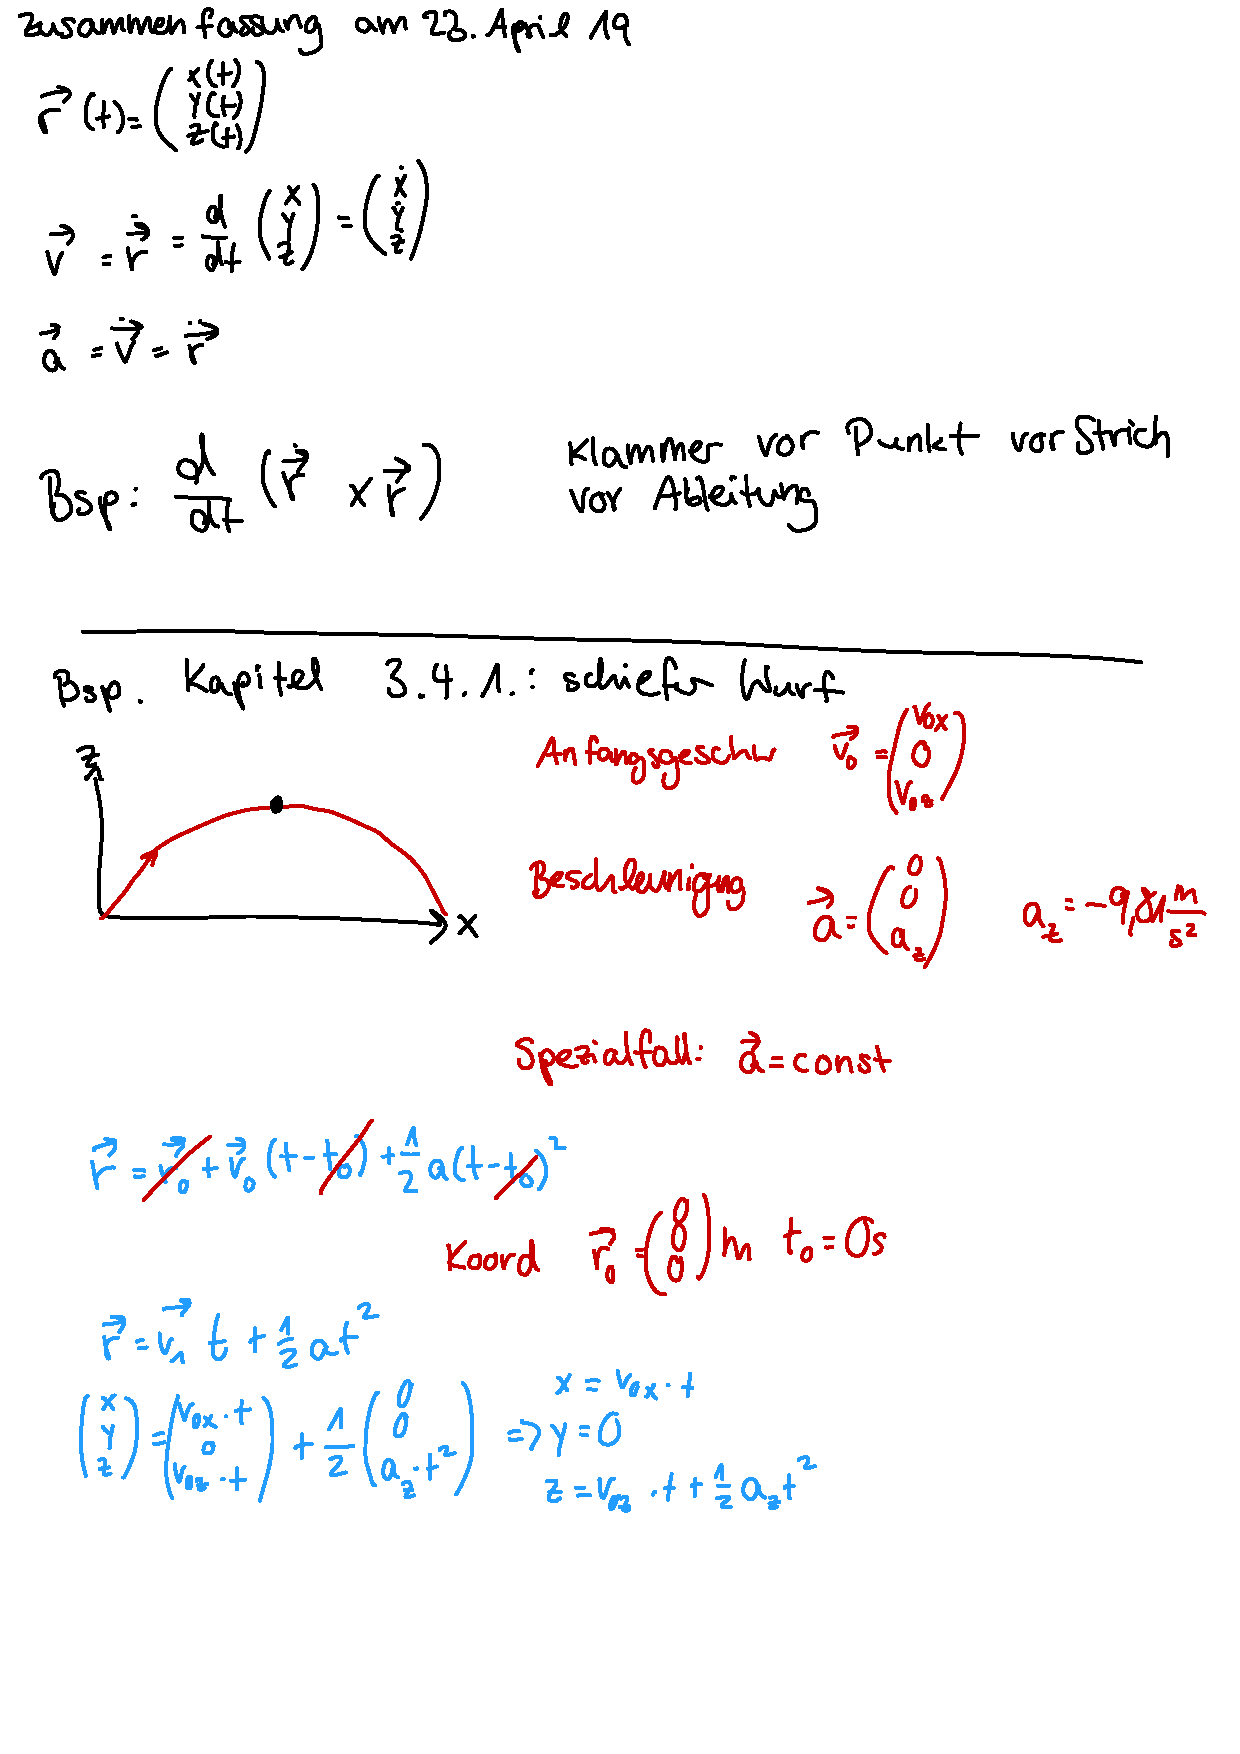
\includepdf[pages=-]{./images/PHY1-19.pdf}
		
		\part{Vorlesung 5}
			\section{Newton Axiome}
				\begin{itemize}
					\item \textbf{Trägheitsprinzip} Ein Körper bleibt in Ruhe oder gleichförmiger Bewegungn wenn keine resultierende äußere Kraft wirkt.
					\item \textbf{Aktionsprinzip} Ein Körper wird in Richtung der resultierenden äußeren Kraft beschleunigt und es gilt \[ \vec{F} = m * \vec{a} \], mit m = Masse des Körpers (Konstant) und $\vec{a}$ der resultierender Beschleunigungsvektor.\\ \textbf{$\vec{F} = \sum \vec{F}_i$}
					\item \textbf{actio = reactio} Die Kräfte treten immer Paarweise auf: Wenn der Körper A eine Kraft $\vec{F}^{(B)}_A$ auf einen Körper B ausübt, dann wirkt eine gleichgroße, aber entgegengesetzte gerichtete Kraft $\vec{F}^{(A)}_B$ von B auf A.\\
					\textbf{$\vec{F}^{(B)}_A =  - \vec{F}^{(A)}_B$}
				\end{itemize}
			\section{Inertialsysteme}
				In einem Intertialsystem gilt \textbf{$F= m * a$} in seiner reinsten Form. Es ist damit ein Bezugssystem, in welchem sich ein kräftefreier Körper gradlinig gleichförmig bewegt. Die \textbf{Newton´schen Axiome} gelten damit \textbf{nur in Intertialsystemen}\\
			\section{Gravitation}
				$ \vec{F}_{1 2} = G \frac{m_1 m_2}{r^2_{12}} \frac{\vec{r}_{21}}{\vec{r_{21}}} $
				$$\vec F_G=m\cdot\vec a_G$$
				$$F_G=m\cdot g$$
				\[ \vec F_{12}=-G\cdot\frac{m_1\cdot m_2}{r^2}\cdot\hat e_{21} \]
				$g$ ist ortsabh\ddot{a}ngig, $m$ ist eine intrinsische Eigenschaft.\\
				Dabei ist $ G = 6,67 * 10^{11} \frac{m^3}{kg s^2}$
					\subsection{Erdbeschleunigung}
				Die Annahme zum Ausrechnen der Erdbeschleunigung ist dass der Masseschwerpunkt im Mittelpunkt der Masse ist.\\
				\[ F_k = G \frac{M_E * m_k}{( r_E + h)12}  \quad h << r_E \]
				\[ F = G \frac{M_E}{r_E^2} * m_k  = g * m_k\]
				$\Rightarrow g = 9.81 \frac{m}{s^2}$\\
				Zum Momentananen Stand besprechen wir dabei nicht die Fluchtgeschwindigkeit. Diese wird aber zu einem späteren Zeitpunkt noch besprochen.\\
				Da die Erde eine so große Masse hat ist die beschleunigung dem entsprechend für uns klein $1 >> a$ wie aus $F = m * a$ folgt.
				\section{Tr\ddot{a}ge und schwere Masse}	
					$ \vec{F} = \frac{d\vec{p}}{dt} = \frac{d}{dt}(m_{tr\ddot{a}ge} * \vec{v}) $\\
					G mit $ \vec{F}_G  = G \frac{m_{1,schwer} * m_{2,schwer}}{r^2} * \frac{\vec{r}_{12}}{r_{12}} = g * m_{schwer}$\\
		Durch Experimente durchgeführt von \textbf{Eötvös }folge $m_{schwer} = m_{tr\ddot{a}ge}$ für alle Stoffe\\
		\[ G \frac{m_{tr\ddot{a}ge} * a}{\frac{m:E m_{schwer}}{r^2}} = konst = \frac{m_{tr\ddot{a}ge}}{m_{schwer} }= \frac{a * r^2}{G * m_E} \]
		\begin{figure}[htbp]
			\begin{minipage}[t]{6cm}
				\vspace{0pt}
				\centering
				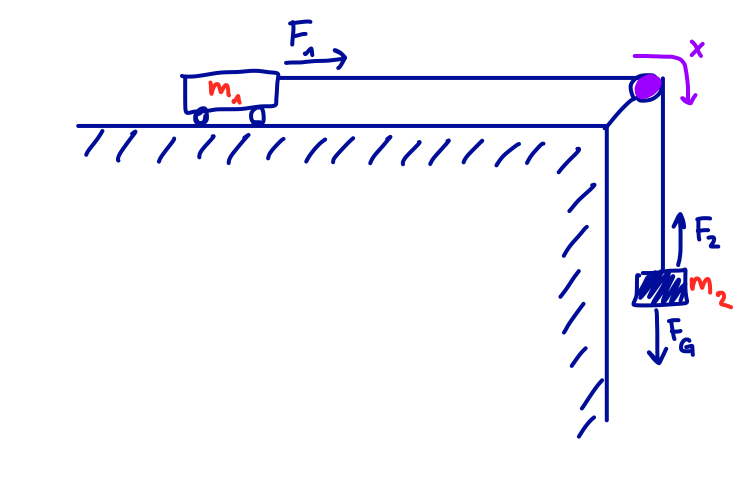
\includegraphics[scale=0.35]{IMG_E8A9C85E8431-1.jpeg}
			\end{minipage}
			\hfill
			\begin{minipage}[t]{6cm}
				\vspace{0pt}
				$ m_1 a_1 = F_1 $ (träge)\\
				$ m_2 a_2 = F_2 + F_G $ (träge)\\
				$ F_1 = - F_2 $\\
				Der Faden muss gespannt bleiben.\\
				$ a_1 = a_2 $\\
				$\Rightarrow m_1 a = - m_2 a $\\
				$ F_1 = -F_2 $\\
				$ m_{1, tr\ddot{a}ge} a_1 = F_1 = - F_2 = -(m_{2, tr\ddot{a}ge} a_2 -F_G) $\\
				mit $ F_G = -m_{2, schwer} g $\\
				$m_{1, tr\ddot{a}ge} a = - m_{2, tr\ddot{a}ge} - m_{2, schwer} g$	\ddot a
			\end{minipage}
		\end{figure}
		\[ a = \frac{m_{2, schwer}}{m_{1,tr\ddot{a}ge} + m_{2,tr\ddot{a}ge}} g \]
				
\end{document}